\chapter{Neural Network Design}
\section{Introduction}
The robot controls its motors using the artificial neural networks and the deep deterministic policy gradient (DDPG) algorithm, produced by Lillicrap et al. The system runs in Python 3, leaning heavily on the TensorFlow library.

\section{Reinforcement Learning Background}
Reinforcement learning (RL) is a subset of machine learning that aims to solve control and action selection problems rather than to perform classification or data clustering. Most reinforcement learning problems involve six main elements: an actor, the environment, rewards, a policy, a value function, and sometimes a model. An actor (sometimes called an agent) takes actions in an environment which returns a state and reward, illustrated in Figure \ref{fig:actor_env_loop}. The actor's primary goal is to maximize the accumulated reward received from the environment. A policy determines which actions the actor takes given the current state and can be considered a mapping from state to action. The value function indicates the long-term reward expected from a state so even if a state only has a small immediate reward, it may possess high value since it leads to high reward states. Some algorithms involve a model of the environment, allowing prediction of the next state from the current state and action. Table \ref{tab:rl_defs} summarizes some common terms and definitions used in the reinforcement learning literature.
\begin{figure}[H]   % [h] means here
	\centering 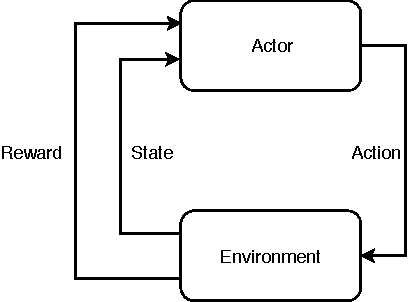
\includegraphics[width=3in, height=3.85in, keepaspectratio]{figures/actor_env_loop.pdf}
	\caption{Actor-Environment Feedback Loop}\label{fig:actor_env_loop}
\end{figure}
Actors strive to maximize the long-term discounted reward, $G_t$, where the subscript $t$ denotes the time step. In RL problems with a definitive end (denoted by $t=T$) such as a game of chess, $G_t$ is finite and can be calculated simply as the sum of all future rewards (\ref{eq:Gt_simple}). 
\begin{equation}
	\label{eq:Gt_simple}
	G_t=R_{t+1}+R_{t+2}+\dots + R_{T}=\sum_{k=t}^{T-1} R_{k+1}
\end{equation}
However, continuous problems such as maintaining the temperature of a refrigerator have no maximum time step and therefore, a possibly infinite $G_t$. The introduction of a discount factor, $\gamma$, makes such a situation manageable. The discount factor weights the worth of future rewards exponentially by their distance into the future. It ranges from 0 to 1 where 0 completely devalues future rewards while a discount factor of 1 weights all future rewards equally. In practice, the discount factor is less than 1 in order to allow $G_t$ to converge \cite{sutton_2017}. The discount factor can be considered a knob setting the algorithm between myopic (short-sighted, only values immediate rewards) and far-sighted (willing to sacrifice immediate reward for greater long-term return).
\begin{equation}
	G_t=R_{t+1}+\gamma R_{t+2}+\gamma^2 R_{t+3} + \dots = \sum_{k=0}^{\infty} \gamma^k R_{t+k+1}
\end{equation}
The value function is the expected long-term reward as function of the state under a certain policy $\pi$ (\ref{eq:value_func}). The $\mathbb{E}_\pi$ operator evaluates the expected value provided the actor follows policy $\pi$.
\begin{equation}
	\label{eq:value_func}
	V_\pi(s)=\mathbb{E}_\pi [G_t | S_t =s]
\end{equation}
Core to many RL algorithms, the Q-function or action-value function is the expected long-term reward as a function of the state \textbf{and action} under a certain policy $\pi$ (\ref{eq:q_func}). The important distinction from the value function is dependency on the action. 
\begin{equation}
	\label{eq:q_func}
	Q_\pi(s,a)=\mathbb{E}_\pi [G_t | S_t =s, A_t=a]
\end{equation}

\LTXtable{\textwidth}{tables/tab_rl_defs.tex}

\section{Reinforcement Learning Algorithms}
Many reinforcement learning algorithms have been applied to control including Q-Learning, State-Action-Reward-State-Action (SARSA), and Deep Deterministic Policy Gradient (DDPG), among others. Note that these methods differ from evolutionary algorithms in that they actively learn as they interact with the environment.

RL algorithms can be classified by their use of models (model-based vs. model-free) and actor policy (on-policy vs. off-policy). Model-based strategies first develop a model of the environment and then use a planning algorithm with the model to create a controller. Model-free algorithms forgo the model entirely and find good policies directly. 

On-policy algorithms learn the policy followed by the actor while off-policy strategies learn a policy different from the one followed by the actor. Various policies exist but the most commonly referred to in the literature include optimal, greedy, $\epsilon$-greedy, and random. The optimal policy $\pi_*$, by definition, produces greater value for every possible state than any other policy $\pi$, expressed in (\ref{eq:optimalpol}) where $\mathcal{S}$ is the set of all possible states. An actor using the greedy policy always takes the action with the highest value or Q-value depending on implementation. The $\epsilon$-greedy policy tells an actor to pick the greedy action with probability $1-\epsilon$ and a random action with probability $\epsilon$. Finally, an actor under the random policy always takes random actions.
\begin{equation}
	\label{eq:optimalpol}
v_{\pi_*}(s) \geq v_{\pi}(s), \forall s \in \mathcal{S}
\end{equation}

\subsection{Q-Learning}
Q-Learning is an off-model, off-policy algorithm that estimates the Q-function of the environment. The Q-function represents the "quality" of every possible action in every possible state. For example, imagine a game of tic-tac-toe as shown in Figure \ref{fig:tictactoe}. Each of the nine spaces can take one of three values (blank, X, or O) so the game has $3^9=19,683$ possible states (although some states are not achievable as the game would end once a player gets three in a row). Given a particular state, the Q-function returns the quality of each possible action the player could take. Therefore, the optimal action to take is simply the one with the highest Q-value. 
\begin{figure}[H]   % [h] means here
	\centering 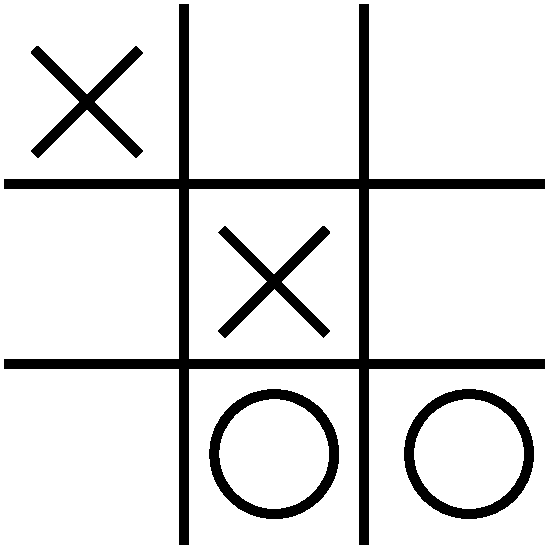
\includegraphics[width=3in, height=3.85in, keepaspectratio]{figures/tictactoe.pdf}
	\caption{A Game of Tic Tac Toe}\label{fig:tictactoe}
\end{figure}
Clearly, the Q-function always exists but not necessarily in an analytic or obvious form. So-called tabular Q-learning methods use a 2-D matrix to represent the Q-function with rows for all possible states and columns for all possible actions. The table is initialized with guesses (or all elements set to 0) and iteratively updated to approximate the true Q-function using the Bellman equation (\ref{eq:bellman}).
\begin{equation}
	\label{eq:bellman}
	Q(s,a)=R(s) + \gamma (\text{max}_{a'}(Q(s',a')))
\end{equation}
To improve convergence, Equation \ref{eq:bellman} is modified to include the learning rate $\alpha$. The pseudocode for Q-learning presented by Sutton is reproduced below. The $\text{max}_{a'}()$ operator maximizes its argument with respect to $a'$.
\begin{center} \begin{tabular}{|p{0.9\linewidth}|}\hline % or any other width
Initialize $Q(s,a)$ arbitrarily. \\
Repeat (for each episode): \\
\qquad Initialize $s$\\
\qquad Repeat (for each step of episode):\\
\qquad \qquad Choose $a$ from $s$ using policy derived from $Q$ (e.g., $\epsilon$-greedy)\\
\qquad \qquad Take action $a$, observe $r$, $s'$\\
\qquad \qquad $Q(s,a)\gets (1-\alpha)Q(s,a) + \alpha [r + \gamma \text{max}_{a'}Q(s',a')]$\\
\qquad \qquad $s \gets s';$\\
\qquad until $s$ is terminal \\
\hline
\end{tabular} \end{center}
Notice the algorithm updates the Q-value, $Q(s,a)$, from the Q-value of the next state and greedy policy action, $\text{max}_{a'}Q(s',a')$, regardless of the policy and action taken by the actor. This characteristic makes Q-learning an off-policy algorithm. The Q-value for a particular state and action only updates when the actor visits said state and action so the actor must still explore (not always take greedy actions) for Q-learning to converge.

Clearly, the tabular Q method quickly becomes unfeasible for more complex problems, especially when the states or actions become continuous rather than discrete. When the action or state spaces are continuous, the algorithm must discretize them, forcing a tradeoff between resolution and tractability. For the tic-tac-toe example, the table would be 19,683 rows by 9 columns for a total of 177,147 Q-values while the Q-value table for a game of chess would possess more elements than there are atoms in the known universe.

\subsection{State-Action-Reward-State-Action (SARSA)}
SARSA is an on-policy algorithm similar which shares many characteristics with Q-Learning. The name comes from the fact that the Q update equation uses the current state and action as well as the next reward, state, and action. The pseudocode for SARSA presented by Sutton is reproduced below:
\begin{center} \begin{tabular}{|p{0.9\linewidth}|}\hline % or any other width
Initialize $Q(s,a)$ arbitrarily. \\
Repeat (for each episode): \\
\qquad Initialize $s$\\
\qquad Choose $a$ from $s$ using policy derived from $Q$ (e.g., $\epsilon$-greedy)\\
\qquad Repeat (for each step of episode):\\
\qquad \qquad Take action $a$, observe $r$, $s'$\\
\qquad \qquad Choose $a'$ from $s'$ using policy derived from $Q$ (e.g., $\epsilon$-greedy)\\
\qquad \qquad $	Q(s,a)\gets (1-\alpha)Q(s,a) + \alpha [r + \gamma Q(s',a')]$\\
\qquad \qquad $s \gets s'; a \gets a'$;\\
\qquad until $s$ is terminal \\
\hline
\end{tabular} \end{center}
Unlike Q-learning, SARSA updates Q-values from the next state and next action $Q(s',a')$, making it an on-policy strategy. Like Q-learning the actor must take exploratory actions for the algorithm to converge.

\subsection{Deep Q Network (DQN)}
Deep Q Networks aim to solve the problem with Q-learning in two ways: the inability to handle situations with large state and action spaces and the inability to generalize learnings to new situations. As mentioned previously, maintaining Q-values for the entire state and action space of a complex problem requires enormous memory. The second problem has to do with how the Q-value table updates. In both Q-learning and SARSA, the algorithms iteratively update Q-values for visited (state, action) pairs. However, to fully update the Q-value table means exploring every possible state and action combination multiple times, a non-trivial task. In other words, the algorithms cannot provide reasonable Q-value estimates for unvisited situations.

To overcome these limitations, DQN replaces the tabular Q concept with a neural network where the inputs are the state and action and the output is the Q-value. The loss function is the squared error between the network output and the target Q-function from Q-learning \cite{Mnih_2015}.

To assist DQN training, Mnih et. al. used a technique called experience replay. As the actor performs its 

\subsection{Deep Deterministic Policy Gradient (DDPG)}





\section{Artifical Neural Network Implementation}

\section{Training}

\section{Testing}

\section{Results}

